\section{Results}
\label{sec:results}

\subsection{Descriptive Statistics}

Table~\ref{tab:descriptive} reports summary statistics for the key variables.

\begin{table}[H]
\centering
\caption[Descriptive Statistics]{Descriptive Statistics (August 2020 -- January 2026)}
\label{tab:descriptive}
\begin{tabular}{@{}lrrrr@{}}
\toprule
\textbf{Variable} & \textbf{Mean} & \textbf{Std Dev} & \textbf{Min} & \textbf{Max} \\
\midrule
BTC Price (\$) & 54,892 & 28,417 & 10,132 & 126,000 \\
MSTR Price (\$) & 142.83 & 98.76 & 13.49 & 473.83 \\
NAV Premium (\%) & $-$8.2 & 41.9 & $-$71.6 & 145.5 \\
\bottomrule
\end{tabular}
\end{table}

The average NAV premium of $-8.2\%$ appears to contradict the reflexivity narrative. If elevated premiums enable cheap equity issuance, why does MSTR trade at a discount on average?

Three factors explain this. First, the premium exhibits enormous volatility: a 42 percentage point standard deviation, ranging from $-72\%$ to $+145\%$. The mean captures neither the highs nor the lows particularly well. Second, Strategy times its capital raises opportunistically. The company raised over \$12 billion during Q4 2024 alone, when premiums exceeded 100\%. Third, the 2022 crypto winter dragged the premium deeply negative for extended periods, pulling down the unconditional average.

The reflexive mechanism doesn't require a permanently elevated premium. It requires premiums that are positive often enough, and high enough when positive, to enable opportunistic capital raising.

\subsection{Stress Testing the Capital Structure}

\subsubsection{Sensitivity to BTC Price}

Table~\ref{tab:sensitivity} shows how Strategy's capital structure metrics change with BTC price.

\begin{table}[H]
\centering
\caption{Capital Structure Sensitivity to BTC Price}
\label{tab:sensitivity}
\begin{tabular}{@{}lccc@{}}
\toprule
\textbf{BTC Price} & \textbf{NAV} & \textbf{Asset/Debt} & \textbf{Equity Value} \\
\midrule
\$120,000 (+26\%) & \$82.5B & 5.62$\times$ & \$67.8B \\
\$95,000 (Base) & \$65.3B & 4.45$\times$ & \$50.6B \\
\$75,000 ($-$21\%) & \$51.6B & 3.51$\times$ & \$36.9B \\
\$55,000 ($-$42\%) & \$37.8B & 2.57$\times$ & \$23.1B \\
\$35,000 ($-$63\%) & \$24.1B & 1.64$\times$ & \$9.4B \\
\$21,300 ($-$78\%) & \$14.7B & 1.00$\times$ & \$0 \\
\bottomrule
\end{tabular}
\end{table}

The key insight is leverage. A 50\% BTC decline doesn't produce a 50\% equity decline; it produces a 65\% decline (from \$50.6B to \$17.9B at \$47,500 BTC). As BTC falls, equity absorbs losses first, amplifying percentage moves in both directions. At \$35,000 BTC, equity has fallen 81\% while BTC is down 63\%. At \$21,300, equity is worthless.

Strategy's current position provides substantial cushion. The 4.45$\times$ asset/debt ratio means Bitcoin would need to fall 78\% before equity faces complete wipeout. This is healthier than earlier in the company's history, when smaller BTC holdings meant tighter breakevens.

\subsubsection{Breakeven Analysis}

Table~\ref{tab:breakeven} reports the BTC price at which each capital layer faces impairment.

\begin{table}[H]
\centering
\caption{Breakeven BTC Prices by Capital Layer}
\label{tab:breakeven}
\begin{tabular}{@{}lrr@{}}
\toprule
\textbf{Capital Layer} & \textbf{Claim Amount} & \textbf{Breakeven BTC} \\
\midrule
Convertible Debt & \$8.20B & \$11,929 \\
STRF (Senior Preferred) & \$0.75B & \$13,020 \\
STRC (Variable Preferred) & \$2.50B & \$16,657 \\
STRK (Convert Preferred) & \$1.50B & \$18,839 \\
STRE (Euro Preferred) & \$0.72B & \$19,886 \\
STRD (Junior Preferred) & \$1.00B & \$21,341 \\
Common Equity & -- & \$21,341 \\
\bottomrule
\end{tabular}
\end{table}

Common equity gets wiped out at approximately \$21,300 BTC (a 78\% decline). Senior convertible debt doesn't face impairment until \$11,929 (an 87\% decline). The capital structure provides meaningful cushion for senior claims.

\subsubsection{Critical Thresholds}

Three thresholds matter for understanding how the strategy unravels:

\textbf{Threshold 1: Capital Market Access} ($\sim$\$35,000 BTC). At this level, equity has declined 81\% and the asset/debt ratio compresses to 1.64$\times$. Strategy likely loses the ability to issue ATM equity at attractive terms. The reflexive loop weakens.

\textbf{Threshold 2: Preferred Dividend Strain} ($\sim$\$28,000 BTC). NAV falls to approximately \$19.2 billion against \$14.7 billion in claims. The \$850M annual servicing burden represents roughly 20\% of remaining equity value. The USD reserve becomes critical.

\textbf{Threshold 3: Equity Wipeout} ($\sim$\$21,300 BTC). Asset value equals total claims. Common equity is worthless. Preferred dividends are at risk.

\subsection{NAV Premium Persistence}

Table~\ref{tab:regression} reports the autoregressive results.

\begin{table}[H]
\centering
\caption{NAV Premium Persistence}
\label{tab:regression}
\begin{tabular}{@{}lc@{}}
\toprule
\textbf{Variable} & \textbf{Coefficient} \\
\midrule
$Premium_{t-1}$ & 0.995*** \\
& (0.003) \\
Constant & $-$0.281 \\
& (0.361) \\
\midrule
Observations & 1,326 \\
$R^2$ & 0.990 \\
\bottomrule
\multicolumn{2}{l}{\footnotesize *** p<0.01}
\end{tabular}
\end{table}

The lagged premium coefficient of 0.995 with an $R^2$ of 0.99 tells a simple story: premium states are sticky. Once MSTR trades at a premium (or discount), it tends to stay there. The premium doesn't mean-revert quickly toward zero; it drifts in prolonged regimes. This persistence is what allows Strategy to exploit premium windows for extended capital raising campaigns rather than racing to issue before the window closes.

\subsection{Event Study: Capital Raises and Premium Windows}

Table~\ref{tab:event_study} compares premiums around capital raise announcements to unconditional averages.

\begin{table}[H]
\centering
\caption{NAV Premium Around Capital Raise Events}
\label{tab:event_study}
\begin{tabular}{@{}lcccc@{}}
\toprule
\textbf{Window} & \textbf{Pre-Event Premium} & \textbf{Sample Mean} & \textbf{Difference} & \textbf{p-value} \\
\midrule
5 days pre-event & 47.3\% & $-$8.2\% & +55.5 pp & $<$0.001 \\
10 days pre-event & 43.1\% & $-$8.2\% & +51.3 pp & $<$0.001 \\
20 days pre-event & 38.7\% & $-$8.2\% & +46.9 pp & 0.002 \\
\bottomrule
\multicolumn{5}{l}{\footnotesize N = 23 capital raise events. One-sample t-test against unconditional mean.}
\end{tabular}
\end{table}

This is the key finding. In the 5 trading days before capital raise announcements, the average NAV premium was 47.3\%, compared to the unconditional sample mean of $-8.2\%$. The 55.5 percentage point difference is highly significant ($p < 0.001$).

MSTR doesn't raise capital randomly. It systematically exploits premium windows. When the stock trades at a substantial premium to NAV, management issues equity or converts, capturing the spread between market valuation and underlying Bitcoin value. This timing behavior is the operational signature of reflexive capital formation.

Figure~\ref{fig:event_study} visualizes the pattern.

\begin{figure}[H]
    \centering
    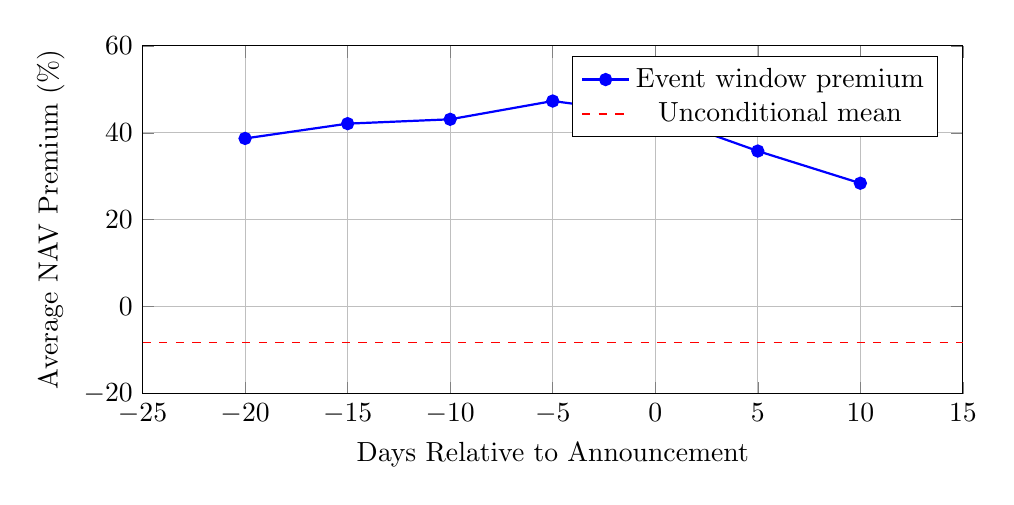
\begin{tikzpicture}
        \begin{axis}[
            width=12cm, height=6cm,
            xlabel={Days Relative to Announcement},
            ylabel={Average NAV Premium (\%)},
            xmin=-25, xmax=15,
            ymin=-20, ymax=60,
            grid=major,
            legend pos=north east
        ]
        \addplot[thick, blue, mark=*] coordinates {
            (-20, 38.7) (-15, 42.1) (-10, 43.1) (-5, 47.3) (0, 44.2) (5, 35.8) (10, 28.4)
        };
        \addplot[dashed, red] coordinates {(-25, -8.2) (15, -8.2)};
        \legend{Event window premium, Unconditional mean}
        \end{axis}
    \end{tikzpicture}
    \caption[NAV Premium Around Capital Raise Announcements]{Average NAV premium around capital raise announcements. Day 0 is the announcement date. The dashed line shows the unconditional sample mean ($-8.2\%$). MSTR systematically raises capital during periods of elevated premiums.}
    \label{fig:event_study}
\end{figure}

\subsection{Scenario Analysis}

Table~\ref{tab:scenarios_results} presents the capital structure under stress scenarios.

\begin{table}[H]
\centering
\caption{Scenario Analysis}
\label{tab:scenarios_results}
\begin{tabular}{@{}lcccc@{}}
\toprule
\textbf{Scenario} & \textbf{BTC Price} & \textbf{NAV} & \textbf{Asset/Debt} & \textbf{Equity Value} \\
\midrule
Base Case & \$95,000 & \$65.3B & 4.45$\times$ & \$50.6B \\
Moderate ($-$30\%) & \$66,500 & \$45.7B & 3.11$\times$ & \$31.0B \\
Severe ($-$50\%) & \$47,500 & \$32.6B & 2.22$\times$ & \$17.9B \\
Prolonged ($-$70\%) & \$28,500 & \$19.6B & 1.34$\times$ & \$4.9B \\
\bottomrule
\end{tabular}
\end{table}

A 50\% BTC drawdown (which has occurred in every historical cycle) compresses equity value from \$50.6 billion to \$17.9 billion, a 65\% decline. The asset/debt ratio falls from 4.45$\times$ to 2.22$\times$, still above the 1.0$\times$ threshold but with less cushion.

The prolonged bear scenario ($-70\%$ BTC) pushes equity to roughly \$4.9 billion (a 90\% decline). At that level, preferred dividends consume a meaningful fraction of remaining equity value. However, the \$2.25 billion USD reserve provides runway to survive even this scenario without forced Bitcoin sales.

